% 
% token_word paper
% Author:  Jason Rohrer
%

%
% Modification History
%
% 2003-February-6  Jason Rohrer
% Created.
%
% 2003-February-13 Jason Rohrer
% Finished initial draft.
% Spell-checked.
% Finished first round of proof reading.
%
% 2003-February-14 Jason Rohrer
% Made changes to match ACM SIG formatting guidelines.
%
% 2003-February-15 Jason Rohrer
% Added changes in response to Jim's comments.
%


\documentclass{acm_proc_article-sp}
\usepackage{graphs}

\newcommand{\tw}{token\_word}

\begin{document}

\title{\tw:\\a Xanalogical Transclusion and Micropayment System}


\numberofauthors{1}

\author{
\alignauthor Jason Rohrer\\
    \affaddr{University of California, Santa Cruz}\\
    \affaddr{Dept. of Computer Science}\\
    \affaddr{Santa Cruz, CA 95064}\\
    \email{rohrer@cse.ucsc.edu}
}

\maketitle



\begin{abstract}
We describe \tw, a web-based xanalogical hypertext system.  
Our system supports almost every core feature associated with Xanadu, an architecture that has been actively discussed for nearly forty years.
Features include deep quotation, unbreakable references, two-way reference chasing, and frictionless micropayments that are backed by real-world currency.
To our knowledge, \tw \ is the first xanalogical system implementation to included all of these features.  Furthermore, \tw \  is the first xanalogical system of any kind to be accessible by a web browser with no additional software.
Previous attempts at full xanalogical implementations took many years and were ultimately never completed.
Given this historical backdrop, an additional contribution of this paper is in analyzing the development strategies that led to a relatively novel success.
A live \tw \  system is running at:

\centering\texttt{http://hypertext.sf.net/token\_word}

\end{abstract}

\category{H.5.4}{Information Interfaces and Applications}{Hypertext/Hypermedia}[Architectures]
\category{K.4}{Computers and Society}{Electronic Commerce}[Payment Schemes]


\terms{Design, Human Factors}

\keywords{Micropayments, quotation, transclusion, Xanadu}

\section{Introduction}
\label{sec:Introduction}
Xanadu has been floating in the collective mind of the hypertext research community for nearly forty years.
Xanadu is a dream and an ideal.  
We know it would be great (or at least interesting) if a xanalogical system existed, but we are also resigned to the notion that such a system will probably never exist.
Is Xanadu impossible?

That question by itself, the impossibility question, is extraordinarily intriguing.  We \textit{know} that Xanadu is not impossible.  
The design, on paper \cite{NelsonLiteraryMachines}, is clear enough:  we just need to build it.  
The problem might be that no one tried to build it.  
But many people did try to build Xanadu over the years.  
The problem might be that the people trying to build it did not have sufficient resources.  But people with extraordinary resources did try to build it.  
Will anyone argue that Autodesk did not have extraordinary software development resources in the late 1980s?  
Furthermore, Autodesk \textit{believed} in Xanadu.  
The following quote from a 1988 Autodesk press release is most telling:

\begin{quote}
In 1964, Xanadu was a dream in a single mind.  In 1980, it was the
shared goal of a small group of brilliant technologists.  By 1989, it
will be a product.  And by 1995 it will begin to change the world.
Much work remains to be done to realize the potential of Xanadu---it
will take the Xanadu development team 18 months to field the first
Xanadu system. \cite{AutodeskPress} 
\end{quote}

In the same press release, Autodesk claimed 1987 sales figures topping \$79 million.  
Indeed, Autodesk had extraordinary resources for its time.  
In 1992, after four years of development and \$5 million spent \cite{AutodeskCost},  Autodesk ceased development of Xanadu \cite{AutodeskPressDrop}.  
Ironically, this decision was made just when the world was ripe for the first global hypertext system \cite{BernersLee92}.

We are scared of Xanadu.  
We hear its siren song and are tempted, but we know that many have tried and many have failed.  
The most frustrating factor is that none of us really know how useful Xanadu would be, even if it \textit{did} exist.  
We can look at architecture diagrams and photographs of cardboard mock-ups \cite{Nelson1999}, but these do not give us a true sense of what it would be like to use a xanalogical system.
Few of us have ever played with a xanalogical user interface prototype, even fewer have paid or received a true micropayment (xanalogical or otherwise), and almost none have transcluded the work of another or had our work transcluded.
Many hypertext systems have been inspired by xanalogical ideas.
To our knowledge, however, none of these system support a true form of transclusion, let alone transclusion \textit{and} micropayments, both of which are central to the Xanadu architecture and user experience.

What is using a xanalogical system really like?
Is it as useful as it sounds?
What made implementing Xanadu so difficult for so many people?  
This paper attempts to answer these question by describing the first fully-realized xanalogical implementation.

Given this historical perspective, the contributions of this paper are threefold.
First, this paper analyzes the process that lead from a paper design to real-world xanalogical software.
Second, this paper shows that modern technology and techniques are of utmost importance for making this implementation process \textit{possible}, let alone quick.
Third, this paper describes a full xanalogical system implementation from the perspective of an end-user.
The novelty of this paper hinges on the implementation, which has a modern flavor, though the underlying ideas are quite old.
We have achieved a novel success, where past attempts have failed, and we feel that the lessons learned from this process are valuable.




\section{The Xanadu Model}

\label{sec:Xanadu}
As mentioned in the above quote, Xanadu's underlying ideas were first incubated by Nelson in the 1960s \cite{Nelson1965}.  
These ideas evolved somewhat over the next forty years, receiving one of their most verbose presentations in Nelson's book \textit{Literary Machines}, which was first published in 1981 \cite{NelsonLiteraryMachines}.  
Nelson's more recent paper on the xanalogical model is up to date in terms of modern technological trends, but the core ideas have not changed \cite{Nelson1999}.  
The high-level description and interpretation of Xanadu given here is based on information culled from \textit{Literary Machines}, Nelson's recent lectures, and personal conversations with Nelson.

The chief goal of Xanadu, distilled into a single phrase, is \textit{frictionless content reuse}.  
This goal would be easily realized in a frictionless, copyright-free world:  authors could simply copy whatever they want and reuse it however they please.  
In our world, however, we have copyright.
Unlike other systems \cite{Clark2000}, Xanadu does not attempt to undermine copyright, but instead tries to work with it. 
All of the design choices and complications in the Xanadu model can be seen as mechanisms for making reuse frictionless in the face of copyright.
When trying to implement unrestricted reuse in a way that works with copyright, we are faced with the following issue:  \textit{copyright forbids unrestricted copying}.

Xanadu's central mechanism is \textit{transclusion}, a form of quotation.  
Transclusion differs from standard quotation in that it does not involve copying of any kind.  
When document $A$ transcludes a quote from document $B$, the quote is stored as a deep reference to the quoted material in $B$:  words from $B$ are not copied into $A$. 
Whenever $A$ is viewed, the words from $A$ are fetched from $A$'s owner, and the necessary words from $B$ are fetched from $B$'s owner.
Thus, even though $A$'s owner has quoted document $B$, the quoted owner still retains control over the distribution and licensing of his or her words.
%Avoiding copying led us to transclusion, and making transclusion work will lead us to the rest of the Xanadu model.

Transclusion creates a serious problem, at least in combination with how we commonly interact with electronic documents.
Electronic documents change constantly.
If $B$ changes or is deleted, $A$'s quote can break.
Xanadu's solution is to forbid document change but encourage document versioning.
Thus, as $B$ is updated, all previous versions are maintained, and $A$'s quote can point to the particular version that $A$'s owner quoted.
Each version of $B$ is immutable, so $A$'s quote will never break.

The Xanadu model refines versioning further by describing an ever-growing, add-only, content space.  
When a document is created, its text is added to this space.
When a document transcludes from another document, it points not to the document itself, but to the transcluded words in the content space.
Thus, a document in Xanadu is a list of pointers to regions in the content space---no text is contained in the documents themselves.
Versioning with this mechanism is particularly space-efficient:  unchanged portions of a new document version can be transcluded from the content space instead of being duplicated.

Along with requiring a new model for document maintenance, transclusion pushes us toward a new model for licensing copyrighted material.
We commonly think about licensing documents only in their entirety.
For example, we may assign monetary value to a printed copy of a book, but we have difficulty imagining how much a chapter, page, or paragraph of that book is worth.
In the Xanadu model, when users read a quote from document $B$ embedded in document $A$, they may only be accessing a small portion of $B$ (for example, a single sentence from a 10,000-word document).
Thus, $B$'s owner must be prepared to license only a portion of $B$ to readers.
The Xanadu model handles this licensing issue with micropayments and per-character values for content.
Nelson is fond of using the term \textit{nanobuck} ($10^{-9}$ dollars) to describe the smallest unit of payment:  documents, or portions of documents, are licensed for $N$ nanobucks per character.
For example, if $N=100$, a document containing one million characters, if licensed in its entirety, would cost \$0.10, while the first half would cost only \$0.05.

When licensing a portion of a document in the Xanadu model, users are actually licensing a region of the content space.
Each character in the content space can be permanently acquired for a one-time licensing fee.
Thus, if users purchase documents that overlap with regions they already own, they only pay for the portions that they have yet to acquire.
Each user accumulates a ``library'' of acquired text regions over time and pays for each region only once.

When a document is accessed that contains quotes from multiple authors, the micropayments are divided and routed to the original authors on a per-character basis. 
Though reading content requires payment, quoting is essentially free, since the content is not accessed during the act of quoting.
In practice, an author will need to read a document before quoting it, but this reading requires only the normal first-access payment, no matter how widely the new, quoting document is expected to be read.
However, the more a document is quoted and read in quoted form, the more micropayments the original author will receive.
Thus, authors benefit from the unrestricted quotation and reuse of their work:  they have no financial motivation for imposing any limits.

We can summarize the Xanadu model with the following feature list:  deep quotation by reference; static underlying content; and per-character, one-time micropayments.


\section{System Architecture}
We designed and built \tw, a full-featured xanalogical system, from scratch in only ten days, and our development team consisted of a single programmer.
To achieve this kind of rapid development, we relied heavily on modern technology and development techniques.
We do not view past Xanadu failures with disdain.
Those early attempts were simply ahead of their time:  the technology of the day was not ready for Xanadu.
The central technologies that made \tw \   development possible were the web, CGI, Perl, and PayPal \cite{paypal}.

Our system, though full-featured, was not designed to be ``the'' scalable xanalogical system that will carry us all into the future.
Instead, we focused on building a usable implementation of core xanalogical features for the purpose of experimentation.
Though scalability was not a design goal, \tw \  was built on top of technologies that have scaled well for other web-based projects \cite{Everything2, WikiWikiWeb, Wikipedia}.
Given these precedents, our architecture could potentially be scalled to support large document collections.
Section \ref{sec:Scalability} discusses these scalability issues in more detail.

\subsection{User Perspective}
In describing the \tw \  user experience, we are faced with the very issue that motivated \tw \  development in the first place:  descriptions in words and pictures do not give us a true sense of what it is like to \textit{use} a system.
Since this paper's focus is on a real-world implementation and not just an abstract description, we encourage readers to visit \texttt{http://hypertext.sf.net/token\_word} to try our system for themselves. 

From the end-user's perspective, \tw \  has many sal\-ient features.
Users access \tw \  with a web browser, and they must create accounts and log in to use the system.  
The central elements of the system are documents, which can contain quotes of other documents.
Quote markers can be hidden or displayed, and quotes can be followed to see the context from which they were taken.
Each document also features a list of documents that quote it, so references can be followed in both directions.
The \tw \   document display interface can be seen in Figure \ref{fig:mainScreen}.

% opera window size for figures:
% 737 x 528
\begin{figure}[t]
\centering
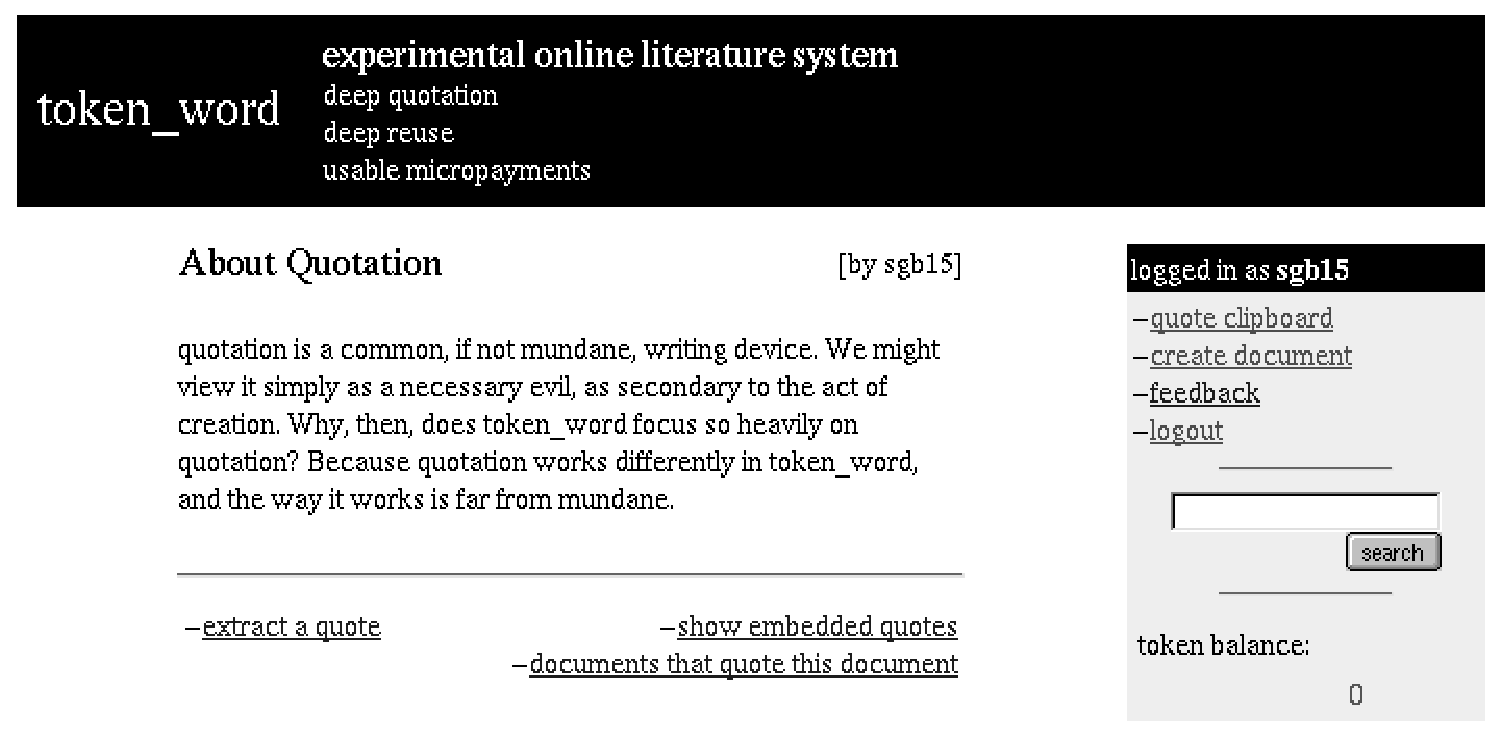
\epsfig{file=images/mainScreen.eps, width=20pc}
\caption{The document display interface.}
\label{fig:mainScreen}
\end{figure}  

Quotes can be extracted from documents and saved to a user's quote clipboard for later reference or use.
To extract a document region as a quote, the user inserts $<$\texttt{q}$>$ $<$$/$\texttt{q}$>$ tags around the desired region in a text area.
This interaction mechanism is arguably more elegant and less error-prone than mouse-based selection highlighting, especially when extracting large regions that span several screens full of text.
Figure \ref{fig:extractQuote} shows the interface for quote extraction. 
Each quote is assigned a $<$\texttt{q N}$>$ tag to be used when inserting the quote into new documents---$<$\texttt{q 3}$>$ refers to the quote at index three on the clipboard.
The use of these abreviated handles hides the complexity of references and document regions from the user.
After extracting a quote, the user never needs to deal directly with the document region again, though the original context of a quote can be seen with a single click from the quote clipboard.
The clipboard interface is shown in Figure \ref{fig:quoteClipboard}.
When creating a new document, a user can enter new text along with handle tags for quotes from his or her quote clipboard, as seen in Figure \ref{fig:docCreate}.
A preview mode shows the new document with all quote references expanded, as seen in Figure \ref{fig:docPreview}.


\begin{figure}[t]
\centering
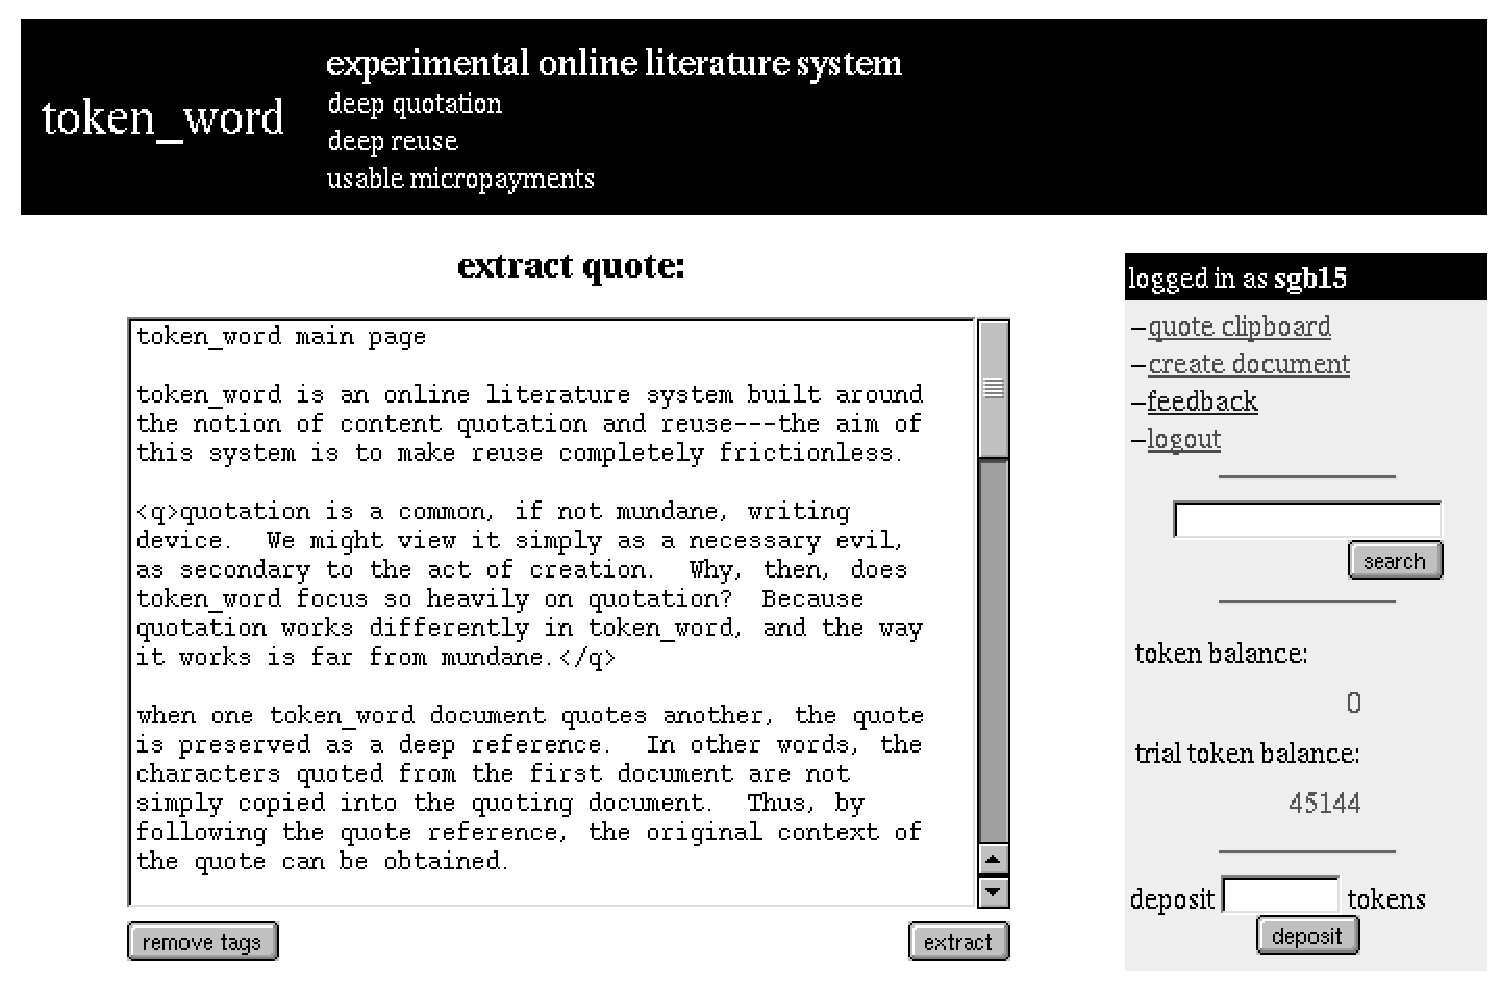
\epsfig{file=images/extractQuote.eps, width=20pc}
\caption{The interface for extracting a quote.  The region surrounded by $<$q$>$ $<$$/$q$>$ tags is selected for extraction.}
\label{fig:extractQuote}
\end{figure}

\begin{figure}[t]
\centering
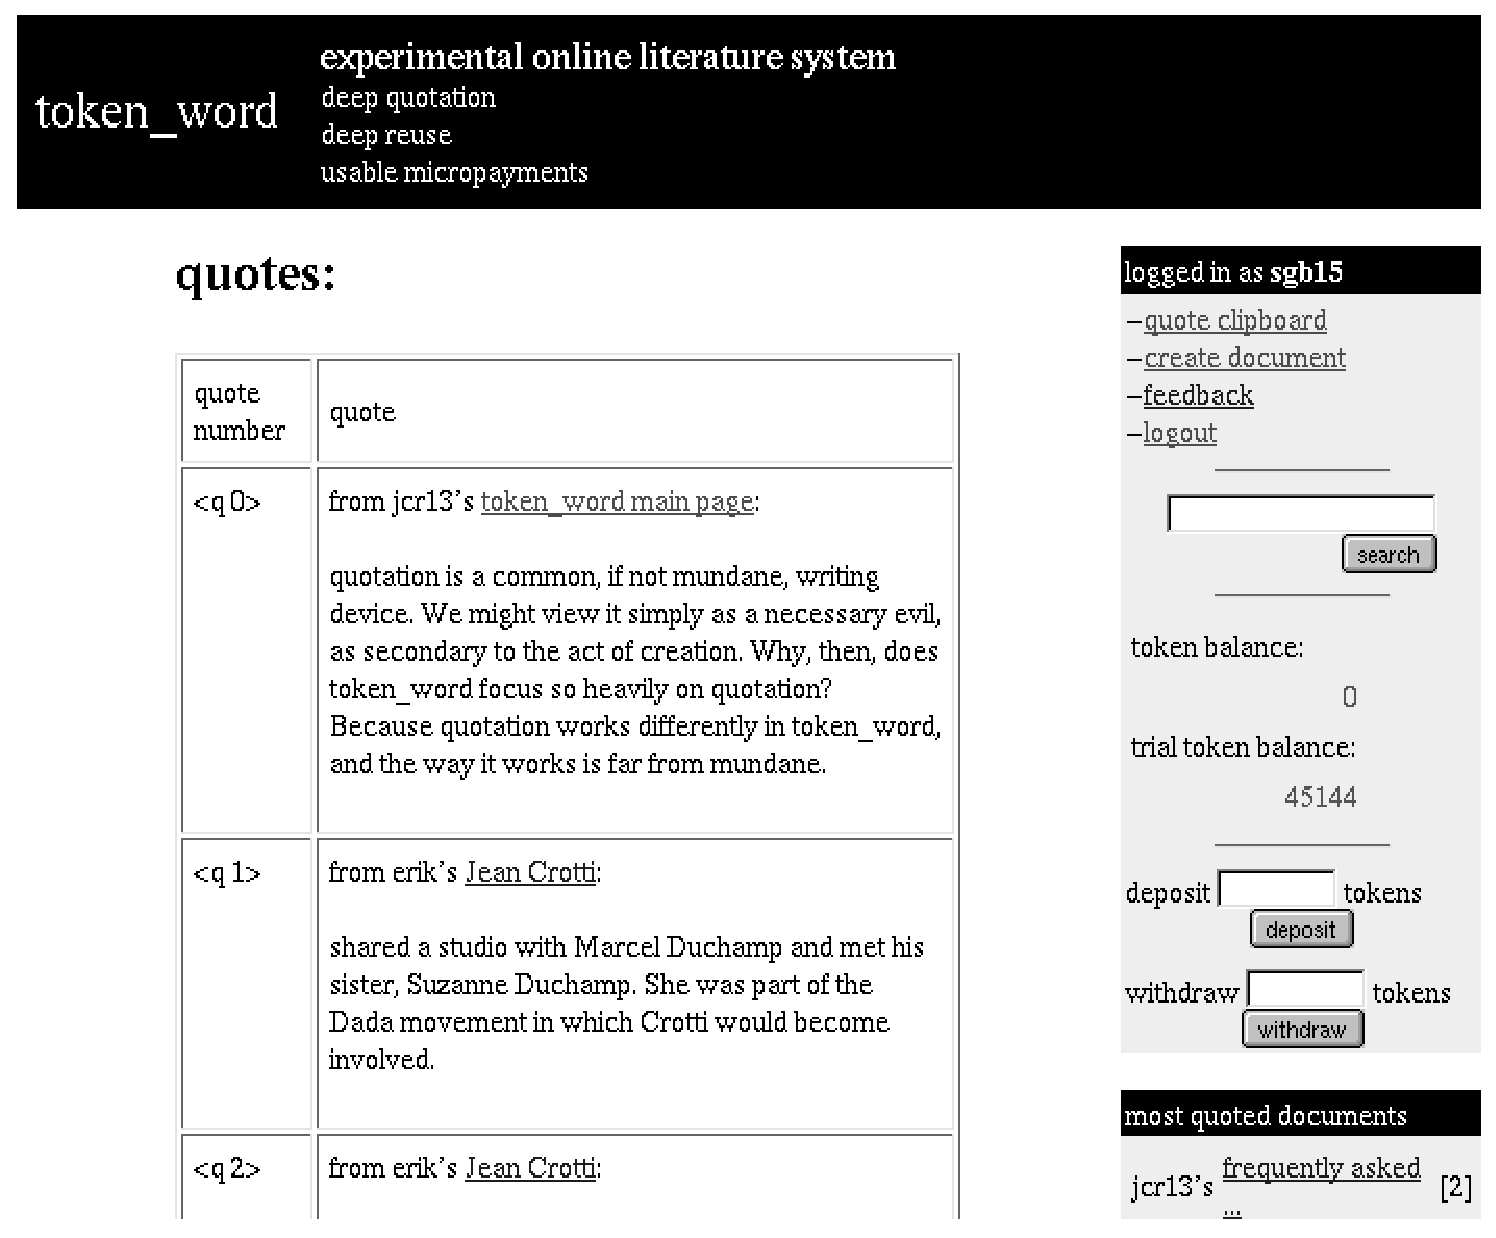
\epsfig{file=images/quoteClipboard.eps, width=20pc}
\caption{The quote clipboard interface.  Each quote is associated with a $<$\texttt{q N}$>$ reference tag, where \texttt{N} is the quote's index on the clipboard.}
\label{fig:quoteClipboard}
\end{figure}

Figures \ref{fig:extractQuote} through \ref{fig:docPreview} show a sequence of actions from a common usage scenareo:  extracting a quote, viewing the quote on the clipboard, creating a new document that uses the quote, and previewing the document.
After correcting the spelling mistake highlithed in Figure \ref{fig:docPreview}, the final step would be to submit the document.
Once submitted, the work becomes a full-fledged \tw \  document, making it readable and quotable by other users in the system.


Each user has a token balance, where one token is worth one character.
The current exchange rate is 1,000,000 tokens for \$1, and Paypal is integrated for token deposits and withdrawls.
When a reader views a document that contains as of yet unviewed text regions, tokens are transfered from the reader to the original authors of the regions.
Users only pay for each piece of text once---repeat viewings of the same text, in any context, are free.
\begin{figure}[t]
\centering
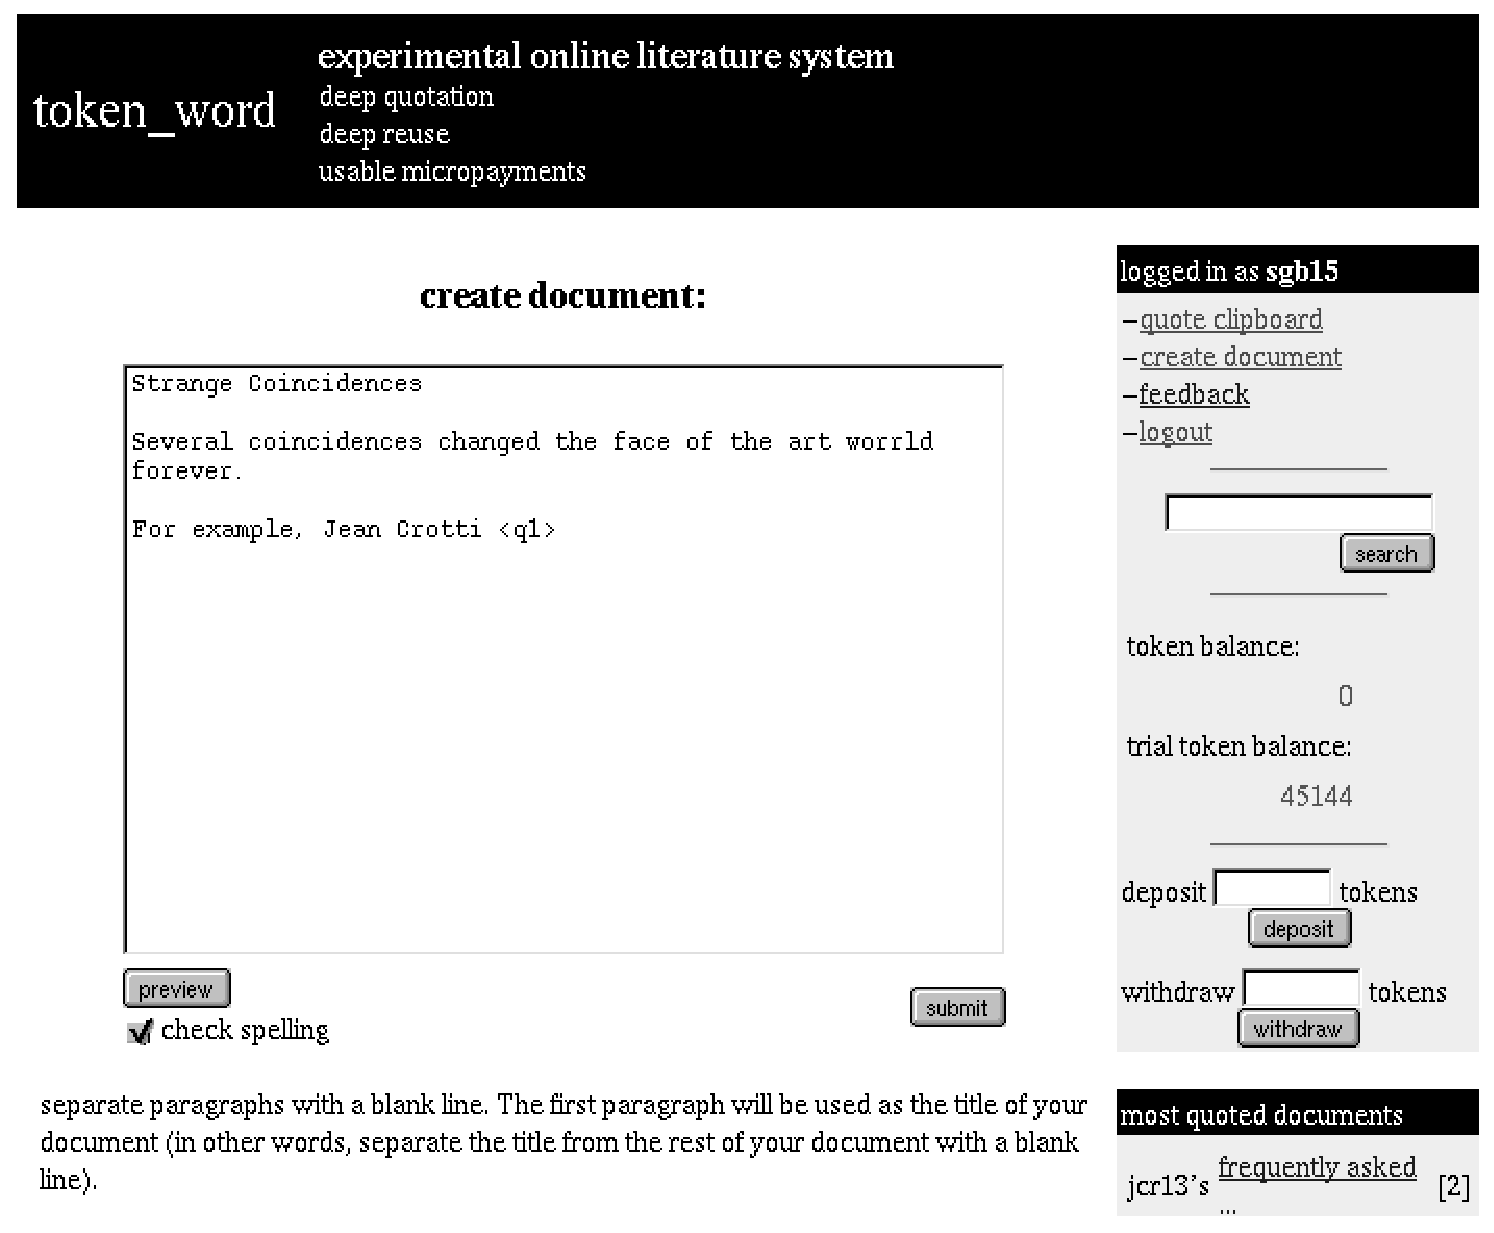
\epsfig{file=images/docCreate.eps, width=20pc}
\caption{The document creation interface. Quote 1 from the clipboard is inserted with the $<$q1$>$ tag.}
\label{fig:docCreate}
\end{figure}

\begin{figure}[t]
\centering
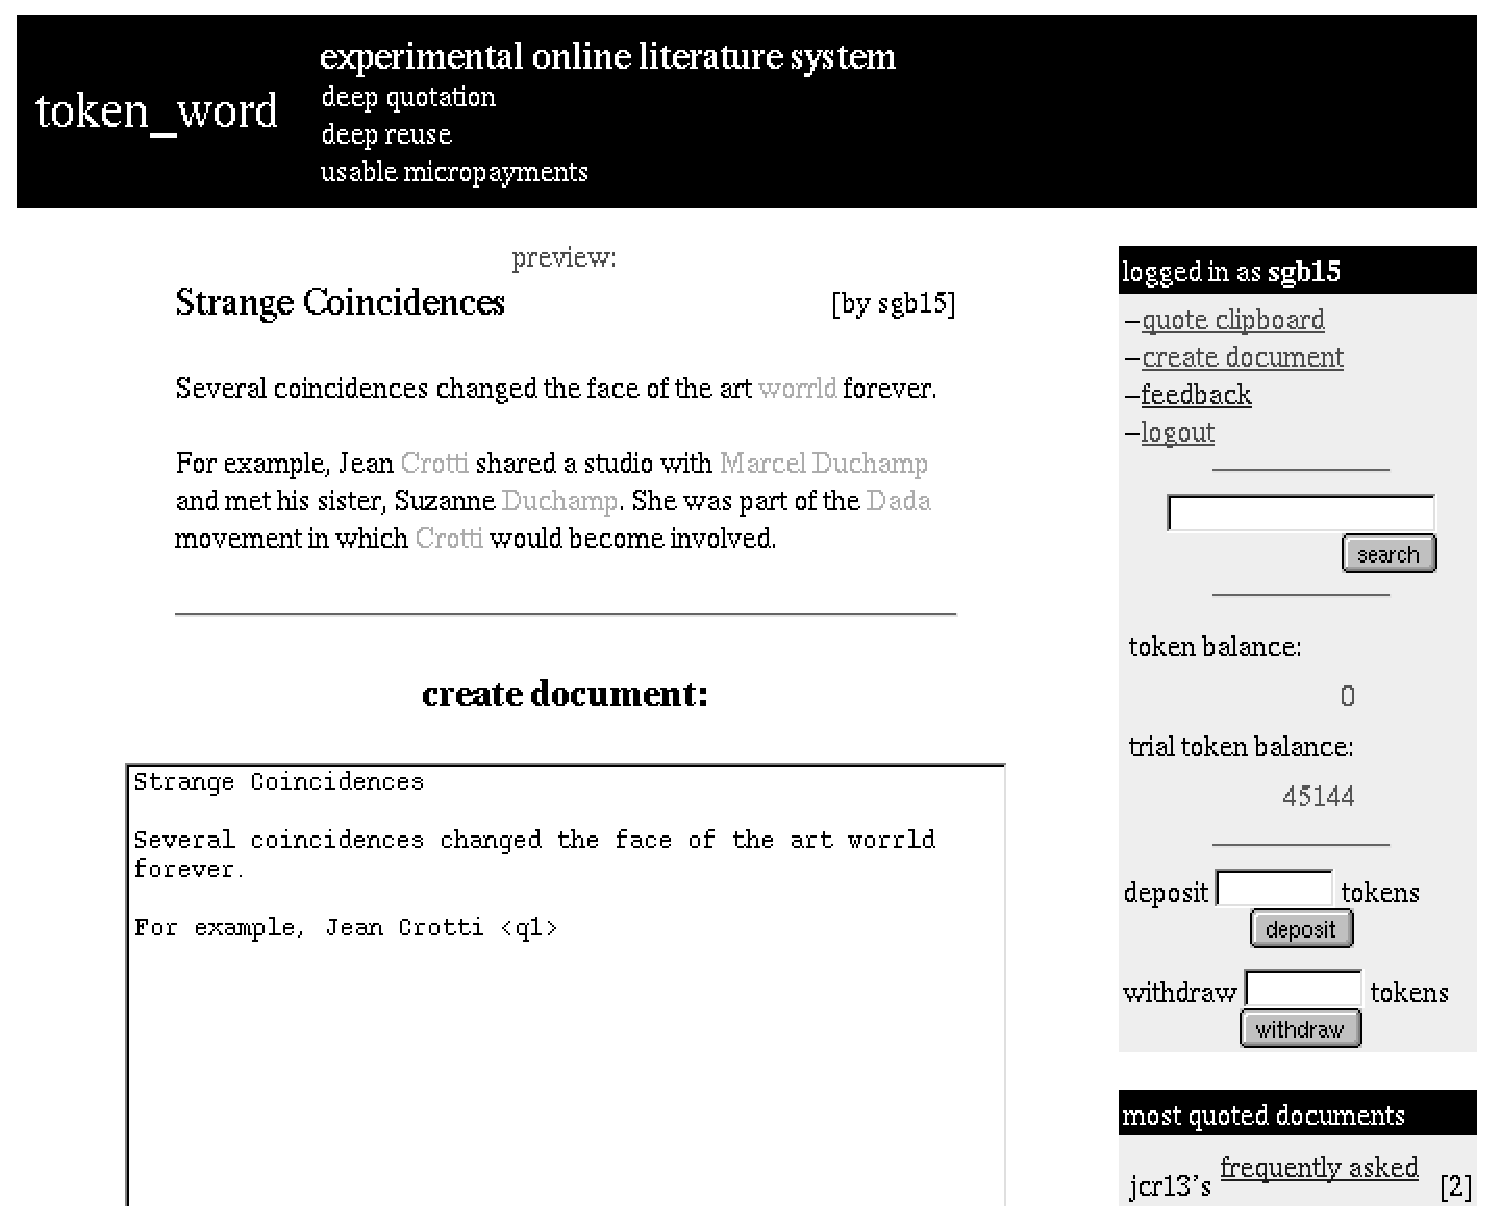
\epsfig{file=images/docPreview.eps, width=20pc}
\caption{The document preview interface.  Quotes are expanded, and possible spelling mistakes are highlighed.}
\label{fig:docPreview}
\end{figure}

Full text searches are supported across the entire document space, and search terms are highlighted when result documents are displayed.
Search results (and other lists in \tw) are sorted with most-quoted documents first, since frequently quoted documents are likely to contain the best information.
This ranking mechanism is similar to Google's PageRank algorithm \cite{Brin1998}. 

\tw \  provides no explicit document linking mechanism.
However, since quote context can be obtained easily, brief quotes can be used to emulate links between documents.
For example, to link to a target document called ``frequently asked questions,'' the title words of the document can be quoted.
When quote markers are shown in the linking document, the words ``frequently asked questions'' will be marked, and clicking on the words will lead to the context of the quote (in other words, to the target document ``frequently asked questions'').
If the title words are not appropriate for use as a link anchor, another more relevant phrase from the body of the target document can be quoted to form a link.
For an example of quotes used as links, see Figure \ref{fig:quotesAsLinks}.

\begin{figure}[t]
\centering
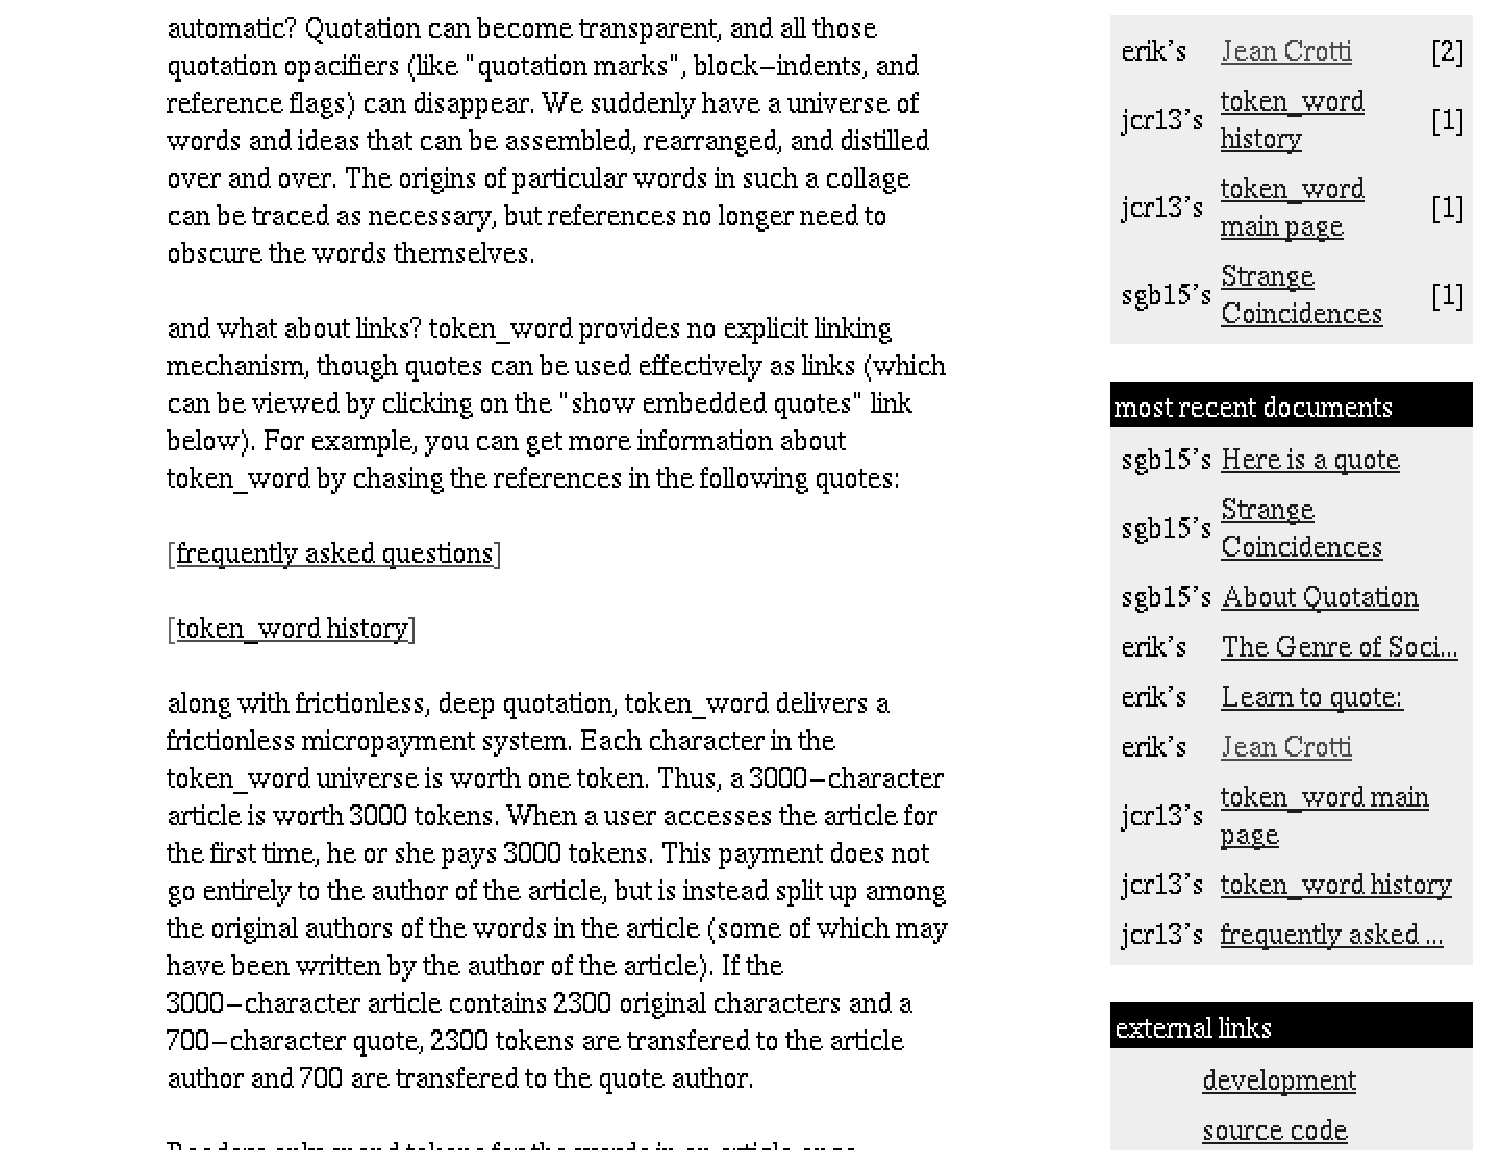
\epsfig{file=images/quotesAsLinks.eps, width=20pc}
\caption{Brief portions of documents can be quoted to emulate links.  Here, the titles of two documents, ``frequently asked questions'' and ``\tw \  history,'' have been quoted.}
\label{fig:quotesAsLinks}
\end{figure}

\subsection{Implementation Details}

\subsubsection{Data Model}
Keeping with the Xanadu model, \tw \  separates documents from the text they contain.
There are two types of data objects in \tw:  documents and chunks.
A chunk contains a raw block of contiguous text, while a document is a list of references to text chunks.
Some of the referenced chunks in a document may have been created at the same time as the document (for new text in the document), while others may be part of quotes taken from other documents.

Each reference in a document contains a pointer to a text chunk region and an optional pointer to a document context region.
The document context pointer tracks which document the material was quoted from and is used for quote reference chasing.
If a document refers to a new text chunk that has not appeared in any previous documents, the document context pointer is omitted:  such chunks are not part of quotes and have no references that can be chased.
With this two-pointer model, we can distinguish ``original'' material in a document from quoted material.  % and support recursive reference chasing.
By following references recursively for a nested quotation, the original author and document context of particular words can be obtained.
%When following a quote reference, a chain of references may need to be chased before the original context of the text is found. 


\begin{figure*}[t]
\begin{center}

\begin{graph}(8,4)(-4,-1.65)
\graphnodesize{0.6}
\graphnodecolour{1}
\opaquetextfalse

\rectnode{A}[1.5,2](-6,0)[\fillednodesfalse]     
\nodetext{A}(0,1.25){Document $A$}
\rectnode{AQuote}[1.5,0.75](-6,.25)[\graphnodecolour{0.5}]  
\rectnode{kInA}[1.5,0.5](-6,.25)[\graphnodecolour{0.85}]
\roundnode{kInAStartAnchor}(-5.25,.5)[\graphnodecolour{0}\graphnodesize{0}]
\roundnode{kInAEndAnchor}(-5.25,0)[\graphnodecolour{0}\graphnodesize{0}]

\roundnode{QuoteInAStartAnchor}(-5.25,.625)[\graphnodecolour{0}\graphnodesize{0}]
\roundnode{QuoteInAEndAnchor}(-5.25,-.125)[\graphnodecolour{0}\graphnodesize{0}]


\rectnode{B}[1.5,2](-2,0)[\fillednodesfalse]
\nodetext{B}(0,-1.25){Document $B$}
\roundnode{kInBAnchor}(-1.45,-.5)[\graphnodecolour{0}\graphnodesize{0.1}]
\rectnode{AQuoteInB}[1.5,0.75](-2,-.5)[\graphnodecolour{0.5}]
\rectnode{BQuote}[1.5,0.5](-2,-.5)[\graphnodecolour{0.85}]

\roundnode{AQuoteInBStartAnchor}(-2.75,-.125)[\graphnodecolour{0}\graphnodesize{0}]
\roundnode{AQuoteInBEndAnchor}(-2.75,-.875)[\graphnodecolour{0}\graphnodesize{0}]

\roundnode{QuoteInBStartAnchor}(-1.25,-.25)[\graphnodecolour{0}\graphnodesize{0}]
\roundnode{QuoteInBEndAnchor}(-1.25,-.75)[\graphnodecolour{0}\graphnodesize{0}]


\rectnode{C}[1.5,2](2,0)[\fillednodesfalse]      
\nodetext{C}(-.75,1.25){Document $C$}
\rectnode{kInC}[1.5,1](2,0)[\graphnodecolour{.85}]
\rectnode{BQuoteInC}[1.5,0.5](2,.125)[\graphnodecolour{0.85}]

\roundnode{BQuoteInCStartAnchor}(1.25,.375)[\graphnodecolour{0}\graphnodesize{0}]
\roundnode{BQuoteInCEndAnchor}(1.25,-.125)[\graphnodecolour{0}\graphnodesize{0}]

\roundnode{kInCStartAnchor}(2.75,.5)[\graphnodecolour{0}\graphnodesize{0}]
\roundnode{kInCEndAnchor}(2.75,-.5)[\graphnodecolour{0}\graphnodesize{0}]



\rectnode{k}[1.5,1](6,0)[\graphnodecolour{.85}]      
\autonodetext{k}[n]{Chunk $k$}
\rectnode{QuoteInK}[1.5,0.5](6,.125)[\graphnodecolour{0.85}]
\roundnode{QuoteInKStartAnchor}(5.25,.375)[\graphnodesize{0}\graphnodecolour{0}]
\roundnode{QuoteInKEndAnchor}(5.25,-.125)[\graphnodesize{0}\graphnodecolour{0}]

\roundnode{kStartAnchor}(5.25,.5)[\graphnodecolour{0}\graphnodesize{0}]
\roundnode{kEndAnchor}(5.25,-.5)[\graphnodecolour{0}\graphnodesize{0}]




\diredge{QuoteInAStartAnchor}{AQuoteInBStartAnchor}[\graphlinedash{4 4}\grapharrowtype{2}]
\diredge{QuoteInAEndAnchor}{AQuoteInBEndAnchor}[\graphlinedash{4 4}\grapharrowtype{2}]
\dirbow{kInAStartAnchor}{QuoteInKStartAnchor}{0.17}[\grapharrowtype{1}]
\dirbow{kInAEndAnchor}{QuoteInKEndAnchor}{0.17}[\grapharrowtype{1}]

\diredge{QuoteInBStartAnchor}{BQuoteInCStartAnchor}[\graphlinedash{4 4}\grapharrowtype{2}]
\diredge{QuoteInBEndAnchor}{BQuoteInCEndAnchor}[\graphlinedash{4 4}\grapharrowtype{2}]

\dirbow{QuoteInBStartAnchor}{QuoteInKStartAnchor}{-0.19}[\grapharrowtype{1}]
\dirbow{QuoteInBEndAnchor}{QuoteInKEndAnchor}{-0.19}[\grapharrowtype{1}]


\dirbow{kInCStartAnchor}{kStartAnchor}{.17}[\grapharrowtype{1}\graphlinecolour{0.65}]
\dirbow{kInCEndAnchor}{kEndAnchor}{.17}[\grapharrowtype{1}\graphlinecolour{0.65}]


\end{graph}

\caption{An example reference chain model.  Dotted lines represent document region pointers, and solid arcs represent chunk region pointers.  Light gray regions represent text from chunk $k$.  Dark gray regions in $A$ and $B$ represent portions of $A$'s quote from $B$ that do not come from chunk $k$ (other chunks have been omitted from this diagram).  Arcs between $C$ and $k$ have been colored gray for clarity.}
\label{fig:referenceChain}

\end{center}

\end{figure*}



For example, suppose that document $A$ quotes a block of text from $B$, and that block contains a quote of original material, residing in chunk $k$, from document $C$.  
$A$'s reference will contain both a pointer to the text chunk $k$ and to the document context $B$.  
$B$'s reference will point to both chunk $k$ and document $C$.  
At the end of this reference chain, $C$'s reference will point only to $k$.
Figure \ref{fig:referenceChain} shows a diagram of our model applied to this reference chain.








Quote clipboards are modeled like documents, but with minor differences.
Each quote on the clipboard points to a contiguous document region.
Since a  document region can be comprised of regions from multiple chunks, we might want to model each quote as a list of references, just like we model a document.
However, we simplify the clipboard by modeling each quote as a single document region pointer with no chunk region pointers.
To insert a clipboard quote into a new document, we can resolve the chunk region references for the quote and set the document region for each of these references to the document from which the quote was extracted.
This simple model allows us both to track the extraction context of the quote and to store the quote clipboard efficiently.
Figure \ref{fig:quoteClipboardModel} shows a diagram of a quote clipboard modeled in this way.
The alternative list model mentioned above could not be easily used to track quote extraction context, and the clipboard representation would be much larger.


\begin{figure}[b]
\begin{center}

\begin{graph}(6.5,2.8)(-3.25,-1.0)
\graphnodesize{0.6}
\graphnodecolour{1}
\opaquetextfalse


\rectnode{q0}[1.0,0.5](0,0)
\nodetext{q0}{$q0$}
\autonodetext{q0}[n]{Clipboard}
\roundnode{q0Anchor}(.5,0)[\graphnodecolour{0}\graphnodesize{0}]
\rectnode{q1}[1.0,0.5](0,-.5)
\nodetext{q1}{$q1$}
\roundnode{q1Anchor}(-.5,-.5)[\graphnodecolour{0}\graphnodesize{0}]


\rectnode{A}[1.5,2](2.5,0)     
\autonodetext{A}[n]{Document $A$}
\rectnode{AQuote}[1.5,0.75](2.5,.25)  
\roundnode{QuoteInAStartAnchor}(1.75,.625)[\graphnodecolour{0}\graphnodesize{0}]
\roundnode{QuoteInAEndAnchor}(1.75,-.125)[\graphnodecolour{0}\graphnodesize{0}]


\rectnode{B}[1.5,2](-2.5,0)     
\autonodetext{B}[n]{Document $B$}
\rectnode{BQuote}[1.5,0.5](-2.5,-.25)  
\roundnode{QuoteInBStartAnchor}(-1.75,0)[\graphnodecolour{0}\graphnodesize{0}]
\roundnode{QuoteInBEndAnchor}(-1.75,-.5)[\graphnodecolour{0}\graphnodesize{0}]



\diredge{q0Anchor}{QuoteInAStartAnchor}[\graphlinedash{4 4}\grapharrowtype{2}]
\diredge{q0Anchor}{QuoteInAEndAnchor}[\graphlinedash{4 4}\grapharrowtype{2}]

\diredge{q1Anchor}{QuoteInBStartAnchor}[\graphlinedash{4 4}\grapharrowtype{2}]
\diredge{q1Anchor}{QuoteInBEndAnchor}[\graphlinedash{4 4}\grapharrowtype{2}]

\end{graph}

\caption{An example quote clipboard model.  Dotted lines represent document region pointers.}
\label{fig:quoteClipboardModel}

\end{center}

\end{figure}






\subsubsection{Data Representation}
The system data is stored in a filesystem directory tree.
Each user has directory that holds that user's chunk files, document files, and quote clipboard files, along with a list of previously purchased chunk regions.
To support two-way reference chasing, each document has a file that tracks the documents that quote it.

References in documents are represented using the following format:
\begin{center}
\texttt{<chunkUserID, chunkID, chunkStartOffset, length;\\ 
docUserID, docID, docStartOffset>} 
\end{center}
The portion of the reference before the ``;'' describes the chunk region of the reference.  
The second portion, which is optional, describes the document region context of the reference.  
Note that \texttt{chunkUserID} may differ from \texttt{docUserID}, since the quoted region may itself be part of a quote in the context document (in the case of a nested quote).
Consider our previous example, which is shown in Figure \ref{fig:referenceChain}, and suppose that documents $B$ and  $C$ are owned by \texttt{userY} and \texttt{userZ}, respectively.
%For example, document $A$ may quote from document $B$, but the portion that $A$ quotes may be part of $B$'s quote from document $C$.
The reference included in document $A$ might look like this:
\begin{center}
\texttt{<userZ, k, 12, 50; userY, B, 125>} 
\end{center}
In other words, we have 50 characters from chunk $k$, starting with character 13, which were quoted from document $B$, starting at character 126.
\texttt{userZ} owns both document $C$ and chunk $k$, since $k$ was created as original material for use in $C$.
Note that \texttt{length} is not specified for the document region context of a reference, since it would be redundant (in our example, it would be 50).

%With this representation, a reference can be used both to fetch the required text chunk region and to display context in case of a followed quote reference.
%By following context repeatedly for a nested quotation, the original author and document context of particular words can be obtained.
%When a new chunk is created as part of a document, the context portion of the reference is omitted, indicating that the document is the first context in which this chunk was used.

As described in our discussion of data models, each quote on a clipboard has only a single pointer to a document region and no chunk region pointers.
We represent these references with the following format:
\begin{center}
\texttt{<docUserID, docID, startOffset, length>} 
\end{center}
Consider our previous example clipboard, which is shown in Figure \ref{fig:quoteClipboardModel}, and suppose that documents $A$ and  $B$ are owned by \texttt{userX} and \texttt{userY}, respectively.
The clipboard representation might look like this:
\begin{center}
\texttt{<userX, A, 37, 75>}\\
\texttt{<userY, B, 100, 50>}\\ 
\end{center}




Since documents and text chunks are static, full text searches can be implemented using an index that is updated in real time as documents are created.
Each word in the index is associated with a list of documents containing that word.
When a document is added to the system, its reference is appended to the end of the index list for each word that it contains.


\subsubsection{Development}
The entire \tw \   system is implemented as a single CGI script written in Perl, though the script is broken up into eight modules for organization purposes.
Perl's built-in support for regular expressions was useful for the rather complicated text processing done by \tw.
Many of these text processing operations can be expressed in succinct and elegant ways using Perl.
For example, highlighting possible misspellings in preview mode was a minor addition that required less than fifteen lines of code.

User interfaces can be layed out easily with HTML, and CGI processing is well-supported by existing Perl modules.
The CGI model requires a stateless action-response programming style, which makes it easy to focus on one feature at a time during development.
Perl-based CGI programming seems to be the modern method of choice for rapidly developing complex, multi-user applications.
Other systems that have used this development method successfully are discussed in Section \ref{sec:RelatedWork}.

Even though the full development cycle was short, we used an iterative process.
Features were added one at a time to \tw, and the system was maintained in a usable form at all times.
For example, we started with a system that managed text chunks, then added document management, then added quotes, and then added tokens transfers.
Final iterations added features such as spell checking and index-based searching.
From our understanding of previous xanalogical implementation efforts, this iterative process may have been key to our success.
The Xanadu model is complex and subtle, and it is easy to get bogged down by details without ever producing a working system.
Our system started out simple and grew in complexity, feature by feature.


\subsubsection{Scalability Limitations}
\label{sec:Scalability}
The main scalability limitation of our implementation is the use of a filesystem as a data backend.
Each text chunk and document are stored in a separate file, and these data objects can be quite small.
A chunk file will be as large as the text it contains, but a document file stores only references.
For example, if a new document is created that references only one new chunk and contains no quotes, the document file will contain a single reference.
The example reference given above was represented using only 33 bytes of ASCII text.

The first limitation is in terms of storage efficiency:  most filesystems have a minimum file size, and this minimum is usually larger than 1 kilobyte.
In our example, 33 bytes of document data would occupy at least a kilobyte of disk space.

The second limitation is in terms of filesystem architecture:  Unix-like filesystems use an inode table, and each file must be associated with a unique inode.
When a filesystem is created, the number of available inodes is fixed, and this number can be relatively small (the common ratio for modern Linux systems seems to be about 200,000 inodes per gigabyte of disk space). \cite{OperatingSystems}
Thus, even if we ignore storage efficiency concerns, our implementation is limited in terms of the number of chunks and documents it can contain.

If our system did need to scale to support millions of users and billions of chunks and documents, several approaches would be possible.
First, we could use an existing database system as a backend to store chunks and documents.
This approach would deal with the inode limitations, and it might actually improve performance, since database queries would replace the directory lookups that are currently used to fetch chunks and documents.
A second approach would be to implement a simple application-level virtual filesystem for chunk and document storage.
With this approach, we could taylor the storage system to our specific needs, though its development would certainly be labor-intensive.

All filesystem operations in \tw \  are wrapped by a single module with only a handful of interface functions.
By modifying the implementation of these module functions, either of the scalable backends mentioned above could be added to \tw \  with no changes to the rest of the code. 

We chose a filesystem backend, despite its scalability limitations, because of its simplicity.
This choice fits into our implementation philosophy, since the focus was on producing a working system and adding features iteratively.
A scalable backend might be seen as a feature to be added in a future iteration.
Our system, in its current form, is still functional in terms of its goal, which is to support exploration of a multi-user xanalogical system.

%\subsection{Xanalogical Improvements}


%\subsection{Missing Features}


\section{Micropayment Issues}
With our micropyament system, we wanted to leverage PayPal's \cite{paypal} immense popularity and familiarity.
By handling real-world currency exclusively through PayPal, instead of through our own virtual money system, we can process payments in a secure and trustworthy fashion.

However, PayPal's currency model does not support the microdollar resolution that we need, so we cannot rely on this service alone for transfering tokens between users.
Even if PayPal did support high-resolution payments, it does not allow a third party to initiate transfers between account holders in a transparent and frictionless way (and for good reason, given the security issues).

To deal with these issues, we built an internal token balance system and used PayPal integration only for deposits and withdrawls of real-world currency.
With this configuration, a deposit is by no means frictionless (logging in to PayPal is required), but after the deposit has been made, token payments are completely transparent as the user accesses \tw \  documents.
Similarly, withdrawing tokens in exchange for real-world currency is not frictionless: 
PayPal does not support an automated payment mechanism, so withdrawl requests must be queued for manual processing by the \tw \  system administrator.
Whereas deposits take effect immediately (using PayPal's ``Instant Payment Notification'' service), withdrawn token refunds are delayed by the response of the human administrator.
From the administrator's point of view, the withdrawl queue can be used to increase security, since any suspicious activity can be investigated before real-world payments are made.  

In our live system, we chose an exchange rate of 1,000,000 tokens for \$1, though this parameter can be changed on a site-by-site basis.
With this exchange rate, we tried to minimize financial burden on readers while still assigning appreciable value to content.
For example, the full text of this paper would cost about \$0.04, so 25 people would need to read it before it earned \$1 worth of tokens.


\subsection{Balancing Risk}
Given that micropayments in \tw \  are mandatory and automatic, a major barrier to system adoption might exist:  trying \tw \  would require the deposit of real-world currency.
Even the main page displayed after login is a first-class \tw \  document, so a new user with no tokens would not even be able to read a description of \tw, let alone try any of its features.

One way of dealing with this adoption barrier would be to give each new user a small number of ``free'' tokens to start with (for example, at least enough tokens to read the main page).
This solution would allow new users to try the system with no monetary investment, but it carries an enormous risk for the \tw \  system administrators.
A small group of users could create many fake accounts and then use each account to read a large dummy document owned by one user.
This kind of scam could be used to consolodate the free starting tokens from many accounts into one account, and then a withdrawl could be made in exchange for a large amount of real-world currency.
Even if users are not trying to intentially scam the system, doling out free tokens poses considerable risk.
One user might write documents that are popular with new users (for example, a collection of how-to documents) and ammass a large number of free tokens over time---the withdrawl of these tokens could financially devastate the \tw \  administrators.

We have devised a risk-free mechanism that deals with the adoption barrier.  
Our approach uses two token types.
The first type of tokens, called \textit{trial} tokens, have no real-world value.
Each new account starts out with a small number of trial tokens (in our live system, each account starts with 50,000 trial tokens).
The second type of tokens, called \textit{real} tokens, can be exchanged for real-world currency.
The token transfer logic in \tw \  keeps track of token types:  trial tokens can only be transfered between users' trial balances, and real tokens can only be transfered between real balances.
Trial tokens are favored, and real tokens are only spent when a user has no trial tokens.

For example, suppose that the balances of three users are as shown in following table:
%suppose user $A$ has a trial:real token balance of 50:200, user $B$ has a balance of 0:500, and user $C$ has a balance of 10:0.
\begin{center}
\begin{tabular}{|l||r|r|}
\hline
User&Trial balance &Real balance\\
\hline
$A$&50 &200\\
\hline
$B$&0  &500\\
\hline
$C$&10 &0  \\
\hline
\end{tabular}
\end{center}
Suppose that user $A$ reads a new 100-chracter document that is owned by $B$, but that the document contains a 20-character quote by $C$.
User $A$ must pay 100 tokens to access this new content, with 80 going to $B$ and 20 going to $C$.
The transfer logic favors trial tokens, so $A$'s trial balance is exhausted first by transfering 50 tokens to $B$.
The remaining payment to $B$ is made with 30 real tokens, and 20 real tokens are also transfered to $C$.
The resulting balances are shown in the following table:
\begin{center}
\begin{tabular}{|l||r|r|}
\hline
User&Trial balance &Real balance\\
\hline
$A$&0 &150\\
\hline
$B$&50  &530\\
\hline
$C$&10 &20  \\
\hline
\end{tabular}
\end{center}


%$A$'s new balance would be 0:150, $B$'s new balance would be 50:520, and $C$'s new balance would be 10:20. 

This two-type scheme allows users to try \tw \  extensively without a monetary investment, and it also poses no financial risks to the administrators.
Note that though trial tokens have no real-world value, they still have value in \tw, since they can always be used to purchase new content.
Inside \tw, a user that amasses many trial tokens is just as wealthy as a user that has many real tokens.
A user that actively publishes popular content in \tw \  could effectively use the system forever without depositing any real-world money.

\section{Related Work}
\label{sec:RelatedWork}

Much of the existing work on xanalogical systems was discussed in Sections \ref{sec:Introduction} and \ref{sec:Xanadu}, so we will focus on related non-xanalogical systems here.

However, we should mention that interest in Xanadu has not waned in recent years, even though development work on Udanax, the last official (and most ambitious) Xanadu implementation effort, ceased in 1995 \cite{Udanax}.
For example, Lukka and Fallenstein describe a system that uses ideas taken from Freenet for xanalogical content storage and retrieval \cite{FreenetXanadu}.
As another example, recent work with XLink has focused on adding transclusion capabilities to the web \cite{Lowe2001}, but support is limited to embedding entire documents.
XPointer can be used in conjunction with XLink to refer to document spans \cite{Vitali2002}, though nothing prevents these references from breaking when documents change.






\subsection{Wikis}

In terms of implementation, \tw \  is closely related to a recent class of hypertext systems known as Wikis, which are often implemented as Perl-based CGI programs.
Wikis are reader-edited web sites, and web-based HTML forms are used as the interface for page authoring.
In many cases, Wikis are open for editing by the public at large.

Despite the fact that their sociological aspects receive most of the attention, Wikis are also interesting from a hypertext perspective.
Links can be created to documents that do not yet exist without knowing where those documents will eventually reside.
To create a new document, a user must follow one of these dangling links in an existing page, which leads to a page creation screen.
Thus, in a Wiki, there is no way to create a page in isolation.
In fact, the name of a new page is determined by the contents of the dangling link and cannot be specified in the page creation screen.

%\tw \  differs from a Wiki in its approach to hypertext, since a \tw \  quote can only be taken from an existing document.
%No mechanism is provided for refering to a document that does not yet exist.


The first Wiki was created by Ward Cunningham in 1995 and is still active today \cite{WikiWikiWeb}.
The most ambitious Wiki-based project is Wikipedia, a user-edited encyclopedia, which recently grew to over 100,000 entries \cite{Wikipedia}.


\subsection{Everything2}
Like \tw \  and Wikis, Everything2 \cite{Everything2} is a web-based hypertext system implemented using CGI and Perl.
Everything2 supports dangling links to pages that do not exist yet, but it handles these links differently than a Wiki does.
When a user follows a dangling link, a search is performed for the title words of the non-existant page.
Thus, dangling links are more fuctional in Everything2 from a reader's point of view.
Using this comparison point, we might conclude that Wikis favor authors, while Everything2 favors readers.
%As soon as a page is created that matches the title of a dangling link, that link points to the new page directly.

In addition to in-line, user-created links (dangling or otherwise), each node in Everything2 features a list of automatically generated links.
These links are culled from user traversal paths:  when a user leaves one page and enters another (either by clicking a link or performing a search), a two-way link is added between the pages.   


\subsection{Weblogs}
Another class of related web based hypertext systems are weblogs, or ``blogs.''
These systems allow content to be added to a web site serially, one post at a time.
Some blogs are used by individuals as a means of sharing daily thoughts with the world, while others aim to be collaborative information spaces and feature moderated comments posted by the public.
One of the most interesting collaborative weblogs is Kuro5hin (pronounced ``corrosion''), which features high-quality news and culture stories submitted and moderated by the public \cite{kuro5hin}.
Many blogs are implemented using CGI and Perl, though more recent efforts seem to favor PHP.


\subsection{Commonalities and Differences}
All three systems discussed above share several features in common with \tw.
First, they are all web-based, collaborative information spaces.
Second, they all rely heavily on existing technology for their implementations.
Third, from what we can tell, they were developed relatively quickly.

In addition, we can see iterative development philosophies in weblogs and Wikis, not necessarily in the individual projects, but in the phenomena themselves.
The first Wikis and weblogs were simple but functional.
Over time, new implementations were released with more features.
Today, the most popular systems in either category are extraordinarily feature-rich.

Of course, out of all of the collaborative information spaces discussed here, \tw \  is the only system that supports deep content reuse and frictionless micropayments.
Thus, these systems are closely related in terms of implementation, but their goals and end-user experiences are very different. 




\section{Conclusion}
Thoughout this paper, we have discussed the strategies that made \tw \  development possible, including an iterative process and heavy use of existing technology.

One additional strategy was crucial, though it has not been mention explicitly:  a focus on a core xanalogical feature set.
We aimed to build a system that supported deep quotation, unbreakable references, and frictionless micropayments---we distilled these features from the Xanadu model in Section \ref{sec:Xanadu}.
However, \textit{Literary Machines} is over 250 pages long, and it is chocked full of features that an ideal xanalogical system might have \cite{NelsonLiteraryMachines}.
Perhaps previous Xanadu efforts aimed to support this entire feature set, and perhaps that is why they failed.

\tw \  is by no means an ideal xanalogical system, and many features are missing.
However, it is still the first system to implement the core features of the Xanadu architecture.
Though one would be hard-pressed to argue that the features included in \tw \  are not crucial, three important features are missing.
First, \tw \  does not explicitly support document versioning.
However, using the quotation primitive, a limited form of versioning can be emulated (a user can quote unchanged regions of the previous version when creating a new version).
Second, \tw \  does not support multi-server integration:  each installation of \tw \  operates in isolation, and quotes between documents at different sites are not possible.
We see multi-server integration as one of the weakpoints in the Xanadu architecture:  how can we ensure that references never break in a system comprised of multiple, separately owned servers?
Even if fault-tolerant, multi-server integration is possible, it is not essential for the end-user experience. 
Third, \tw \   does not support side-by-side document comparission with \textit{transpointing} lines, a classic Xanadu interface feature that Nelson's recent paper describes in detail \cite{Nelson1999}.
The transpointing interface would be difficult, if not impossible, to support in a web browser with no additional software.
However, a side-by-side document comparisson interface, using colored highlighting to indicate itentical regions, has been contemplated for \tw.
Implementing such an interface would be easy, though coming up with a highlighting scheme that works correctly in the general case (for example, without running out of readable colors) is quite difficult.

In recent personal conversations, Nelson has described a layered presentation model that could work in conjunction with a xanalogical storage system.
For example, a presentation layer could specify font sizes, links, or annotations, and multiple layers could be stacked when rendering a particular piece of content.
Given \tw's current data model and presentation logic, adding layers would not be difficult.
In fact, particular types of layers are already implemented:  highlights for misspellings, quote context, and hit search terms are applied to document text after it is assembled.
Highlights are achieved by inserting presentation tags (in this case, HTML font color tags) around particular character spans.
Many other presentation styles could be supported in this way by inserting other tag types.
Layers are an ideal feature to add in a future development iteration.

\section{Acknowledgements}
Thanks are due to Ted Nelson and Jim Whitehead for their contributions to interesting xanalogical discussions over the past year. ``Xanadu'' is a trademark of Ted Nelson.  To prevent confusion, the generic terms (\textit{e.g.}, xanalogical system) have been used wherever possible.

\bibliographystyle{abbrv}
\bibliography{paper}

\end{document}